% Report — belief-critic restoration. pdflatex report.tex (twice)
\documentclass[11pt]{article}
\usepackage[margin=0.9in]{geometry}
\usepackage{lmodern}
\usepackage[T1]{fontenc}
\usepackage{amsmath,amssymb,amsthm}
\usepackage{booktabs}
\usepackage{graphicx}
\usepackage{enumitem}
\usepackage{microtype}
\PassOptionsToPackage{hyphens}{url}
\usepackage[hidelinks,
  pdftitle={Where Actor-Critic Converges Under Partial Observability: An Exactly Solvable Case},
  pdfauthor={Idil Gozel}]{hyperref}
\usepackage{xurl}
\usepackage{multicol}
\graphicspath{{../report_figs/}}

\setlength{\parindent}{0pt}
\setlength{\parskip}{2.8pt}
\setlength{\emergencystretch}{2em}

\newtheorem{proposition}{Proposition}
\newtheorem{lemma}{Lemma}
\newcommand{\keq}{k_{\mathrm{eq}}}
\newcommand{\Jml}{J_{\mathrm{ml}}}
\newcommand{\E}{\mathbb{E}}

\title{\bfseries Where Actor--Critic Converges Under Partial Observability:\\An Exactly Solvable Case}
\author{Idil G\"ozel\\ \normalsize University College London}
\date{July 2026}

\begin{document}
\maketitle

\begin{abstract}
\noindent We study where actor--critic learning converges when the critic cannot observe the
hidden state. In a family of continuous-control POMDPs with linear--Gaussian hidden dynamics,
we solve the learning dynamics exactly. The coupled critic--actor fixed point of the
expected update, the \emph{learning equilibrium}, is obtained in closed form, and it detaches
from the optimum of the actor's own policy class. For Gaussian hidden drives the equilibrium
gain is pinned to the agent's sampling period ($\keq \cdot h = \chi$); at deployment, in the
sampling limit, its cost equals $r\Theta K(0)$, where $K(0)$ is the zero-lag intensity of the
environment's memory kernel --- and this cost ceiling is far more universal than the gain
location, holding across non-Gaussian drives (a numerical finding). The bias is governed by one
algorithmic scalar: the bootstrap parameter $\lambda$, with the equilibrium collapsing onto the
class optimum once the return horizon covers the hidden timescale. Predictions were committed
before the corresponding experiments; standard PPO (CleanRL implementation, five seeds per
configuration) reproduces the causal role of bootstrapping, the equilibrium cost at the observed
exploration, and the location of the $\lambda$-transition. At $\lambda = 0.9$ with exploration
pinned, the iterates overshoot the equilibrium instead of parking at it; we state this
mean-field-to-algorithm gap as a scope limit.
\end{abstract}

\section{Problem and contributions}

Actor--critic methods are used routinely in partially observable environments, and it is well
understood that they can lose performance there. What is not characterized is \emph{where they
converge}: existing theory establishes that a critic blind to hidden state is biased, and
bounds the bias, but does not locate the fixed point the learning dynamics settle into, its
cost, or the conditions that remove it. Throughout, ``converge'' names the rest point of the
\emph{expected} (mean-field) update; whether finite-step stochastic iterates reach it is a
separate question we return to in \S\ref{sec:limits}. In the vocabulary of the
function-approximation literature, bootstrapping and function approximation are known to
interact badly; this report concerns their third interaction, with partial observability. In
our setting this interaction can be solved exactly rather than bounded.

Our contributions, each stated at its proven scope:

\begin{enumerate}[leftmargin=1.6em,itemsep=2pt]
\item \textbf{We prove} the learning equilibrium in closed form for a linear memoryless actor
with Gaussian exploration and a TD(0)/LSTD critic over quadratic observable features, in a
linear--Gaussian family with exact zero-order-hold sampling, under mean-field (expected-update)
semantics: the critic's fixed point (Proposition~\ref{prop:critic}), the actor's expected
update (Proposition~\ref{prop:actor}), and their joint rest point, which lies far from the
optimum of the actor's own policy class.
\item \textbf{We prove}, in the sampling limit $h \to 0$ at deployment, that for Gaussian
hidden drives the equilibrium gain obeys $\keq\, h = \chi(s_e/\Theta K(0))$ and its cost
converges to $r\Theta K(0)$ (root existence proven; uniqueness verified numerically over six
decades; the multi-mode extension is a verified sketch). The cost ceiling extends beyond the
Gaussian family; the gain location does not (\S\ref{sec:scope}).
\item \textbf{We compute} the equilibrium exactly as a function of the bootstrap parameter
$\lambda$, locating the collapse onto the class optimum, and \textbf{we observe} standard PPO
land on the computed values in experiments whose predictions and pass/fail criteria were
committed before launch (five seeds per configuration). The clean agreement holds for
$\lambda \ge 0.95$; the $\lambda = 0.9$ overshoot is stated as a scope limit
(\S\ref{sec:limits}).
\item \textbf{We observe} a phenomenon not predicted in advance: agents given sufficient input
memory start at the restored solution and are later captured by the learning equilibrium as
their exploration noise decays. We state it as an empirical finding with a committed kill
test, not as a theorem.
\end{enumerate}

\section{Setting and the learning equilibrium}

\paragraph{Environment.} The agent observes and controls one coordinate $v$; a hidden mode $z$
it never observes drives $v$:
\[
dv = (z+u)\,dt, \qquad dz = (-\gamma z - c\,v)\,dt + \sigma\,dW, \qquad \sigma^2 = 2\Theta\gamma c,
\]
observed and actuated every $h$ time units through exact zero-order-hold sampling, with cost
rate $qv^2 + ru^2$ discounted at rate $\rho$. Marginalizing $z$ (the Mori--Zwanzig projection
\cite{zwanzig,mori}) is what makes this a POMDP: the hidden mode acts on $v$ as a memory kernel
$K(\tau) = c\,e^{-\gamma\tau}$, in general $K(\tau)=\sum_i c_i e^{-\gamma_i \tau}$ with
timescales $\{\gamma_i\}$ and zero-lag intensity $K(0)=\sum_i c_i$. The behavior policy is
$u = -kv + \eta$, $\eta \sim \mathcal N(0, s_e)$; deployment sets $s_e = 0$. Two reference
values are exact for every instance: the belief-optimal cost $J^\ast$ (Kalman filter plus
certainty-equivalent control \cite{kalman,astrom}) and the best memoryless cost $\Jml$ at gain
$k^\ast$. At the default instance ($c{=}0.3$, $\gamma{=}1$, $\Theta{=}1$, $q{=}r{=}1$,
$h{=}0.05$, $\rho{=}0.05$): $J^\ast = 0.1989$ and $\Jml = 0.2196$ at $k^\ast = 1.649$. The
policy-class gap is therefore 10.4\%, and we verified separately that it is not amplified by
horizon, initial-condition conditioning, or risk-sensitive objectives. Whatever follows is not
a representation effect.

\paragraph{Algorithm.} A standard actor--critic \cite{konda}: the critic is the TD(0)/LSTD
fixed point \cite{sutton88,lstd} over observable features $(1, v, v^2)$; this is the correct
class, since true value functions here are quadratic. The actor follows the score-function
gradient with the critic as baseline \cite{williams}. In the stationary closed loop all
variables are jointly Gaussian, so both objects reduce, by Isserlis' theorem, to polynomials
in the stationary covariances $m_2 = \E[v^2]$ and $x = \E[v v']$ ($v'$ the next-step sample);
we write $\tilde q = q + rk^2$, $\nu = h s_e$, and $\beta = e^{-\rho h}$ (the per-step
discount).

\begin{lemma}[stationarity pins the observed mean reversion]\label{lem:pin}
In the stationary closed loop, for any gain $k$ and any environment parameters,
$\E[v\dot v] = -\nu/2$; in discrete time, exactly,
$m_2 - x = \tfrac{\nu h}{2}\,(1-\kappa/2)^{-1}$ with $\kappa = kh$.
\end{lemma}

The hidden mode resupplies the energy the control removes; that is what stationarity means.
The observed process therefore carries almost no trace of the control effort. A critic restricted
to $v$ must attribute the resulting persistence somewhere, and the only place its feature
class permits is value curvature.

\begin{proposition}[the critic's fixed point]\label{prop:critic}
The TD(0)/LSTD fixed point over $(1,v,v^2)$ has $\theta_1 = 0$ and, exactly at every $h$,
\[
\theta_2 = \frac{h\,\tilde q\, m_2^2}{m_2^2 - \beta x^2}
\;\xrightarrow{\,h\to0\,}\; \frac{\tilde q\, m_2}{\nu + \rho m_2},
\qquad\text{vs.}\qquad
\theta_2^{\mathrm{true}} \approx \frac{\tilde q}{2k+\rho}.
\]
At the default instance, at $k = k^\ast$: $\theta_2 = 16.7$ against a true conditional
curvature of $1.10$ (verified against an independent solve to $1.5\times10^{-13}$).
\end{proposition}

\begin{proposition}[the actor's expected update]\label{prop:actor}
$\hat g(k) = 2hrk\,m_2 - 2\beta\theta_2\, x\, g$, where $g$ is the one-step zero-order-hold
response of $v$ to $u$ ($g \to h$ as $h\to0$). Substituting Proposition~\ref{prop:critic} and
using $x \to m_2$, $g \to h$ in the sampling limit, the continuum equation
$rk = \beta\theta_2(k)$ has no solution for any $k$: the expected update never changes sign.
\end{proposition}

Proposition~\ref{prop:actor} gives the score-function update's expectation \emph{including
scale}, not merely up to a constant: with the critic pinned at its fixed point, an independent
estimate of $\hat g(k)$ matches the closed form to 0.2--2\% (ratios $1.000/1.019/0.988$ at
$k = 1.65/3/6$). The joint rest point of critic and actor is the \emph{learning equilibrium}: a
fixed point of the expected-update dynamics, and a stationary point of no objective (``phantom
equilibrium'' as a gloss). It exists only through time discreteness, at $\keq = 24.8$ for the
default instance against $k^\ast = 1.649$. Figure~\ref{fig:mech} shows the expected-update
field and the confirmation that matters most: stochastic runs initialized \emph{at} the true
optimum leave it along the computed field. Six independent chains all leave $k^\ast$
monotonically, reaching $k = 4.82 \pm 0.03$ by 1.2M steps; the mean-field trajectory over the
same protocol reaches $6.02$, so the chains track the field's shape but lag it by ${\sim}20\%$
--- the online critic trailing its instantaneous fixed point as $k$ moves, which is the open
stochastic-approximation question flagged in \S\ref{sec:limits}. The same algorithm given a
full-state critic stays at the class optimum, so the effect is aliasing, not discounting bias.

\begin{figure}[t]
\centering
\begin{minipage}[b]{0.46\textwidth}\centering
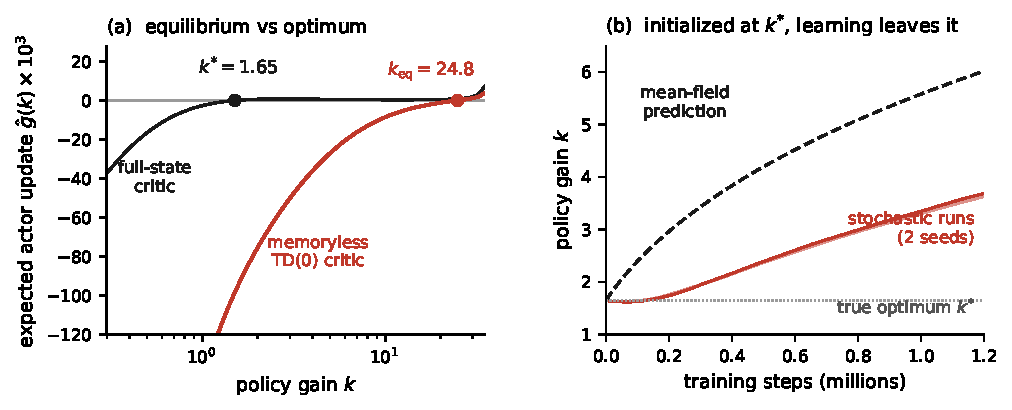
\includegraphics[width=\textwidth]{R1_mechanism.pdf}
\end{minipage}\hfill
\begin{minipage}[b]{0.39\textwidth}\centering
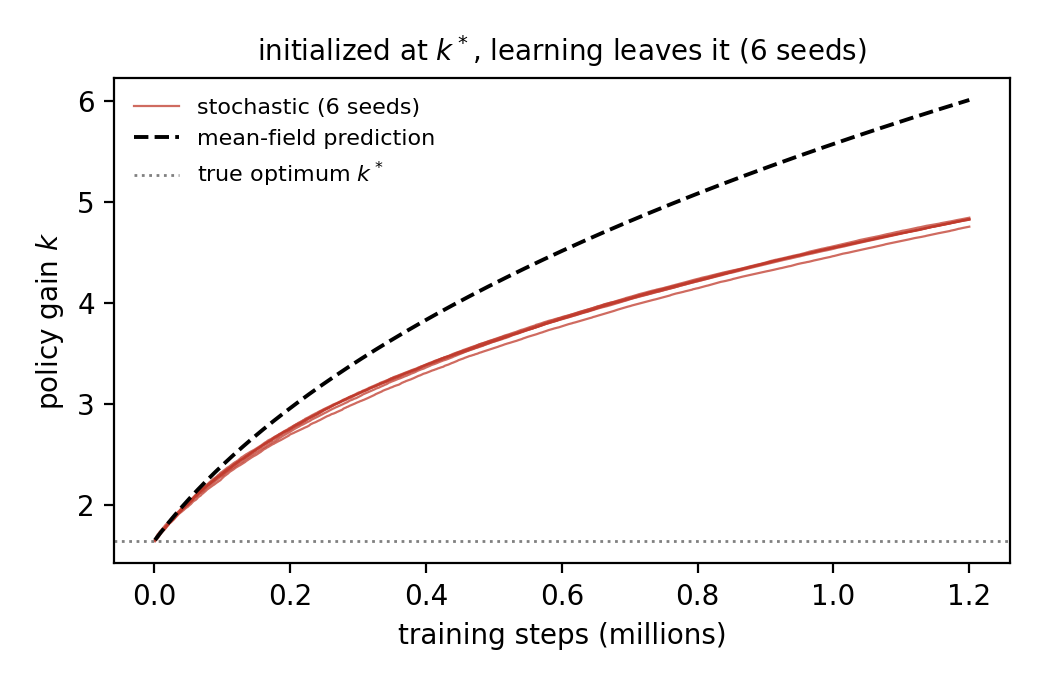
\includegraphics[width=\textwidth]{fig1b_drift_6seeds.png}
\end{minipage}
\caption{(a) Expected actor update under the memoryless TD(0) critic (red) and the full-state
critic (black); zeros marked. (b) Online TD(0) actor--critic initialized at $k^\ast$, six
independent chains (versus the earlier two-seed inset in the left panel), against the mean-field
trajectory: all six leave $k^\ast$ monotonically to $k = 4.82 \pm 0.03$ at 1.2M steps, the
field reaching $6.02$; chains lag the field ${\sim}20\%$. \textbf{We compute} the field
exactly; \textbf{we observe} the iterates track it.}
\label{fig:mech}
\end{figure}

\section{Where the equilibrium sits, and what it costs}

\begin{proposition}[sampling-scale law; Gaussian drives]\label{prop:chi}
Rescale $k = \kappa/h$ and let $h\to0$, $\beta\to1$. The stationary moments have limits
$m_2 = h^2 M(\kappa)$, $x = h^2 X(\kappa)$ with
$M = \Theta c/\kappa^2 + s_e/(\kappa(2-\kappa))$, $X = (1-\kappa)M + \Theta c/\kappa$, and the
equilibrium condition becomes $M^2 - X^2 = \kappa X M$, whose root
$\chi \in (0,2)$ depends on the environment only through $s_e/\Theta K(0)$. Hence
$\keq = \chi/h$: the equilibrium is set by the agent's sampling period. (Existence proven;
uniqueness verified numerically over $s_e/\Theta K(0) \in [10^{-3}, 10^3]$.)
\end{proposition}

\begin{proposition}[cost at the equilibrium; deployment, sampling limit]\label{prop:cost}
At $s_e = 0$ and $h \to 0$ at fixed $\kappa = \chi$, the average cost rate satisfies
$J(\keq) \to r\,\Theta K(0)$. The multi-mode extension (the same per-mode computation;
cross-mode covariances $O(h^2)$) is a verified sketch: numerics agree to 1--3\% across kernel
shapes and $N \in \{1,2,3\}$.
\end{proposition}

Figure~\ref{fig:chi} verifies Proposition~\ref{prop:chi} across fourteen Gaussian-drive
environments, varying $h$, $\gamma$, exploration, kernel shape, and mode count. All fourteen
collapse onto the single curve $\chi$. Two consequences frame the rest of the report. The cost
depends on the kernel only through its zero-lag intensity $K(0)$, while the policy-class gap
depends on the kernel's timescales; the two are therefore governed by different functionals of
the same environment (\textbf{we conjecture} nothing about their correlation sign, which varies
across the family). And since $\keq = \chi/h$, raising the control frequency worsens the failure
linearly.

\begin{figure}[t]
\centering
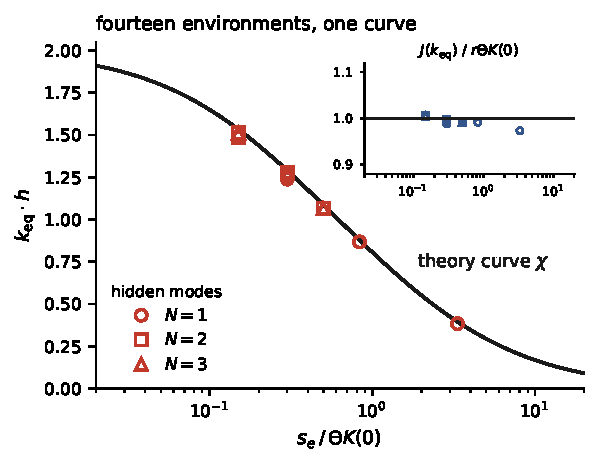
\includegraphics[width=0.50\textwidth]{R3_chi_collapse.pdf}
\caption{Equilibria computed independently at fourteen Gaussian-drive instances against the
curve $\chi$; inset: $J(\keq)/r\Theta K(0)$. \textbf{We compute} both; no fitting.}
\label{fig:chi}
\end{figure}

\paragraph{Scope of the two laws: cost is more universal than gain.}\label{sec:scope}
The $K(0)$ law for the \emph{gain} is a Gaussian-family statement, and the in-family evidence
above could not have shown otherwise. The aliased critic converts the \emph{persistence of
observable energy} ($v^2$, quasi-statically $\zeta^2$) into value curvature; for a Gaussian
hidden drive $\zeta$ the energy autocovariance is $\mathrm{Cov}(\zeta_0^2,\zeta_\tau^2)
= 2C(\tau)^2$, so $C(0)$ and $\mathrm{Var}(\zeta^2)$ are confounded across the entire Prony
family --- the fourteen-instance collapse is consistent with a $K(0)$-only reading \emph{and}
with an energy-fluctuation reading. A deconfounding test (three stationary drives with
\emph{identical} autocovariance $0.3\,e^{-\tau}$; Table~\ref{tab:bath}) separates them: the
equilibrium gain moves $3.4\times$, ordered by $\mathrm{Var}(\zeta^2)$, while the deployed cost
stays within 1\% of $r\,C(0)$ for both unbounded baths and within 7\% for the sub-Gaussian one.
We therefore split the transfer claim into a proven cost ceiling and a Gaussian-only gain law,
and state a three-way target:
\begin{itemize}[leftmargin=1.4em,itemsep=1pt]
\item[\textbf{A1}] (cost, general): for stationary ergodic drives $J(k)\to r\,C(0)$ as $\kappa$
grows --- a transduction/energy-balance identity, no Gaussianity; \textbf{conjecture} with a
derivation sketch from the unit-root identity plus quasi-static moments.
\item[\textbf{A2}] (gain, Gaussian): $\keq\,h = \chi(s_e/C(0))$ for all stationary Gaussian
drives with completely monotone covariance --- the target theorem (density of Prony mixtures in
that class plus continuity of the fixed point), \emph{not yet proven}.
\item[\textbf{A3}] (non-Gaussian, conjecture): at fixed $C$, $\keq$ is set jointly by $C(0)$
and the covariance structure of $\zeta^2$ (zero-lag and timescale); today's three points are
consistent, not yet a law.
\end{itemize}

\begin{table}[t]
\centering
\caption{Deconfounding test (\texttt{bath\_universality.py}): three drives with identical
$C(\tau)=0.3\,e^{-\tau}$, default instance. Pipeline validated on OU ($\keq = 24.62$ vs the
exact $24.79$, 0.7\%). A \emph{numerical finding} motivating the restated scope, not a theorem:
the gain location tracks $\mathrm{Var}(\zeta^2)$; the cost ceiling ($r\,C(0)=0.300$) does not.}
\label{tab:bath}
\small
\begin{tabular}{lccccc}
\toprule
bath & marginal & $\mathrm{Var}(\zeta^2)$ & $\keq$ & $\keq\,h$ & $J(\keq)$ \\
\midrule
telegraph $\pm\sqrt{0.3}$ & two-point (sub-Gaussian) & $0$ & $8.75$ & $0.438$ & $0.280$ \\
OU & Gaussian & $2C(0)^2 = 0.18$ & $24.62$ & $1.231$ & $0.299$ \\
$\sqrt{0.15}\,(w^2{-}1)$ & $\chi^2$-like (skewed) & $\approx 14C(0)^2 = 1.26$ & $29.88$ & $1.494$ & $0.298$ \\
\bottomrule
\end{tabular}
\end{table}

\section{The bootstrap horizon, and the verification}

The TD(0) analysis extends exactly to LSTD($\lambda$)/GAE($\lambda$) critics
\cite{sutton88,lstd,boyan,gae}: the fixed point and expected update close as resolvent
expressions, and \textbf{we compute} $\keq(\lambda)$ exactly. The equilibrium persists while
the return horizon $(1-\beta\lambda)^{-1}$ is short of the hidden timescale $(\gamma h)^{-1}$
and collapses onto the class optimum once it is covered; at the default instance the collapse
falls between $\lambda = 0.95$ and $0.99$. Eligibility traces are the exact cure, and the theory
locates the crossover in advance. This is the quantitative content that folklore (``use longer
returns under partial observability'') does not carry.

\paragraph{Verification protocol.} All external runs use a line-for-line mirror of CleanRL
\texttt{ppo\_continuous\_action} \cite{ppo,cleanrl} on the default instance, five seeds and 10M
steps per configuration; every quantitative prediction and its pass/fail criterion was
committed in writing before launch, including kill criteria that would have retracted the
deep-RL claims. The two $\lambda = 0.9$ numbers below describe different exploration regimes of
the same $\lambda$ and should not be read against each other: with exploration \emph{learned},
the memoryless agent settles near the ceiling as its $\sigma^2$ collapses; with exploration
\emph{pinned} at $0.09$, it overshoots into instability. Two results carry the section
(Table~\ref{tab:pred}, Figure~\ref{fig:lambda}):

\emph{The controlled sweep.} With exploration pinned at $\sigma^2 = 0.09$ by design, the
$\lambda$-sweep landed on the computed transition: median $J = 0.3007$ at $\lambda = 0.95$
against the ceiling $0.300$; $0.223 \pm 0.003$ and $0.221 \pm 0.006$ at $\lambda = 0.99$ and
$0.999$ against the class optimum $0.2196$; collapse between $0.95$ and $0.99$ as computed.
At $\lambda = 0.9$ the pinned-exploration runs do not park at the equilibrium but overshoot
into instability (all five seeds diverge). We report this as observed; the equilibrium's
stability under PPO's finite step sizes is an open question, not a claim.

\emph{The causal pair.} Memoryless PPO at $\lambda = 0.9$ deployed at
$J = 0.3105 \pm 0.011$ with implied gain $8.5$; the identical agent at $\lambda = 1$ (Monte
Carlo targets; same network, same data, bootstrapping off) deployed at $J = 0.226 \pm 0.003$,
gain $1.8$. Neither kill criterion triggered. One caveat travels with this result wherever it
is quoted: the committed window $[0.26, 0.31]$ failed on the high side; the agent's learned
exploration had collapsed to $\sigma^2 \approx 1\times10^{-4}$, at which the theory places the
equilibrium cost at the ceiling $r\Theta K(0) = 0.300$, which the data bracket. This is a
post-hoc reading; the controlled sweep above was designed to test it, and did.

\paragraph{What each experiment constrains.} Deployed cost saturates near the ceiling over a
broad band of high gains, so cost agreement is weak evidence for the equilibrium's location;
implied gain is the sharp probe. The controlled sweep constrains both, since its points sit on
the computed curve. The causal pair constrains cost only: its implied gain (8.5) had not
reached $\keq$ when exploration collapsed, and we make no gain claim for it.

Belief-based repair was tested in the same protocol (asymmetric critics: actor sees $v$,
critic additionally receives a noisy hidden-state estimate): at $\lambda = 0.9$ all noise
types restore at 3\% relative error (gains $1.3$--$3.3$, five seeds each), and at
$\lambda = 0$ the computed noise-type ordering is reproduced: fresh error worse than smooth
error, smooth worse than none.

\begin{table}[t]
\centering
\caption{Predictions against outcomes. ``Committed'' = frozen in writing before the run.}
\label{tab:pred}
\small
\begin{tabular}{p{5.6cm}p{3.4cm}p{4.6cm}}
\toprule
prediction & committed & outcome \\
\midrule
memoryless $\lambda{=}0.9$ converges far above its class optimum; $\lambda{=}1$ twin does not
& before launch; window $[0.26,0.31]$, with kill criteria & $0.3105 \pm 0.011$ (gain 8.5) vs.\ $0.226 \pm 0.003$
(gain 1.8); window missed high (text) \\
$\lambda$-transition between 0.95 and 0.99 at $\sigma^2{=}0.09$ & computed exactly; run
designed for it & collapse between 0.95 and 0.99; $0.3007$ at the $0.300$ ceiling \\
restoration under asymmetric critics at $\lambda{=}0.9$, all noise types at 3\%
& before launch & restored; gains $1.3$--$3.3$ (5 seeds each) \\
noise-type ordering at $\lambda{=}0$ (fresh $>$ smooth $>$ none) & before launch & reproduced \\
equilibria across 14 instances collapse onto $\chi$; $J(\keq) \to r\Theta K(0)$
& closed forms precede numerics & worst deviation 5\% ($\chi$), 1--3\% (cost) \\
\bottomrule
\end{tabular}
\end{table}

\begin{figure}[t]
\centering
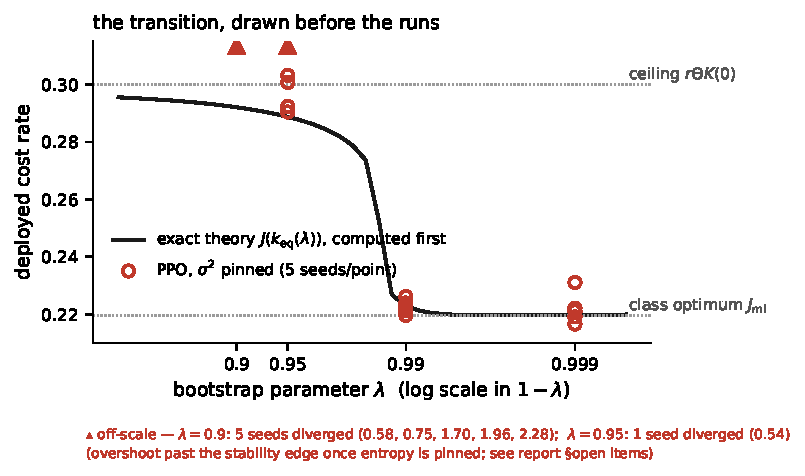
\includegraphics[width=0.54\textwidth]{R2_lambda_flagship.pdf}
\caption{The exact theory curve $J(\keq(\lambda))$ at $\sigma^2 = 0.09$ (line, computed
first) against pinned-exploration PPO (points, five seeds per $\lambda$). Divergent seeds (all
five at $\lambda = 0.9$; one of five at $\lambda = 0.95$) are off-scale; see \S\ref{sec:limits}.}
\label{fig:lambda}
\end{figure}

\section{An observation: restoration by input memory is metastable}

One result was not predicted. Agents were given a 32-frame observation stack, a window longer than the hidden timescale
and sufficient in principle. They begin training \emph{at} the restored
solution ($J = 0.22$--$0.26$ at 0.33M steps, five of five seeds) and are then captured by the
learning equilibrium, reaching the ceiling with implied gains 7--33 by 10M steps
(Figure~\ref{fig:capture}). Capture co-times with the collapse of the learned exploration to
$\sigma^2 \approx 2\times10^{-4}$; an otherwise-similar agent in a second implementation that
retained $50\times$ more exploration stayed restored. Proposition~\ref{prop:chi} suggests the reading: shrinking $s_e$ strengthens the
equilibrium's pull, so below the $\lambda$-threshold the restored solution is only
metastable. Memory in the input is not memory in the credit assignment. \textbf{We conjecture} this and commit the kill test: the
same configuration with $\sigma^2$ pinned at $0.09$ should show no capture.

\begin{figure}[t]
\centering
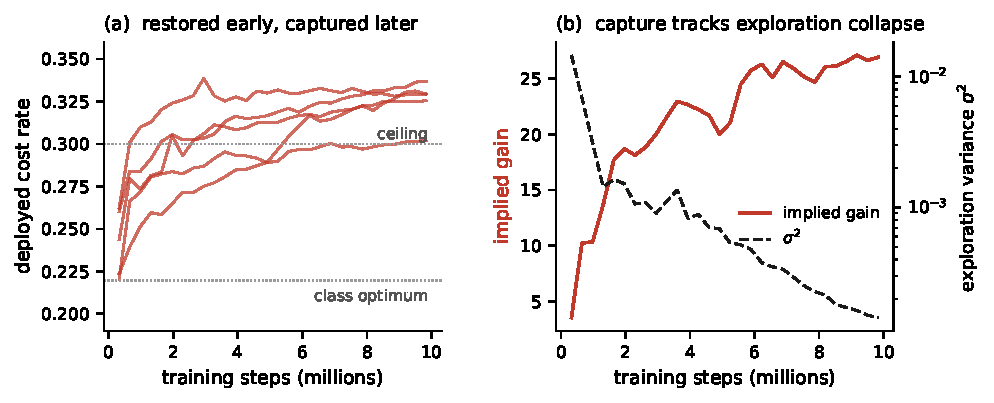
\includegraphics[width=0.72\textwidth]{R4_capture.pdf}
\caption{(a) Five 32-frame-stack seeds: restored early, captured later. (b) Implied gain
against learned exploration variance (one seed): capture tracks entropy collapse.}
\label{fig:capture}
\end{figure}

\section{Relation to prior work}

That memoryless TD learning under partial observability can converge to poor or nonexistent
fixed points is classical \cite{sjj,perkins}; that TD with function approximation converges to a
projected, biased fixed point under full observability is equally classical \cite{tvr}; and the
asymmetric actor--critic literature proves that state-blind critics are biased and bounds the
resulting error terms \cite{baisero,lambrechts,cayci}. The existence question is sharper than
``poor or nonexistent'' suggests: for a \emph{continuous} exploration strategy a fixed point is
\emph{restored} (Brouwer; our Gaussian policy qualifies), whereas $\varepsilon$-greedy
discontinuity can destroy it \cite{perkins}; badness is fixed by neither, and in that same study
the non-convergent $\varepsilon$-greedy agent out-earned the convergent softmax one --- a 2002
precedent for convergence and quality dissociating. Filter-stability analyses give finite-memory
Q-learning guarantees under observability conditions \cite{kara}, a complementary regime. To our
knowledge, the object computed here has not previously been obtained in closed form: the
location, cost, and parameter dependence of the actor--critic learning equilibrium under partial
observability, with the condition that removes it; a systematic search protocol accompanies this
report and the claim is stated at that scope.

\section{What this does not show}\label{sec:limits}

The committed plateau window for the causal pair failed high; the resolution (exploration
collapse) is stated wherever the result is quoted and was confirmed by the controlled sweep.
The mean-field-to-algorithm gap is a scope limit on contribution 3, and the reason the title's
``converges'' is a statement about the expected-update field, not the iterates: the equilibrium
is attracting under the mean-field dynamics at both TD(0) and $\lambda = 0.9$ (the expected
update crosses zero from below at $\kappa = 1.24$ and $1.03$), yet under pinned exploration at
$\lambda = 0.9$ PPO's finite steps destabilize \emph{on the approach} and it is never attained
--- a finite-step effect near the inner loop's stability edge, not a repelling rest point, whose
quantitative treatment is a named next computation. The bath-universality result
(\S\ref{sec:scope}) is a numerical finding, not a theorem: the squared-OU bath confounds skew
with kurtosis, the $\zeta^2$ timescale differs across baths, and each $(\text{bath},k)$ was
evaluated once (tight SEs, $\le 4\times10^{-5}$). Belief-noise damage at $\lambda = 0$ differs
between our two implementations --- ruinous versus mild, identical ordering --- and is under
diagnosis. Transfer beyond the family, tested on velocity-masked MuJoCo, was inconclusive
(control baselines destabilized under high $\lambda$), and we make no transfer claim. The proven
scope is a scalar memoryless policy with deterministic emission of $v$; the named next
computations are the two-feature actor (exactly solvable here), observation noise, and the
capture kill test above.

\paragraph{Artifacts.} Complete proofs with executable machine-precision verifications
(\texttt{theorem/formal\_proofs}), all experimental records with per-run time courses
(\texttt{theorem/empirical\_evidence}, \texttt{results/}), the frozen prediction documents,
the drift and bath-universality reproduction scripts, and the environment and agent code
accompany this report in the repository
\url{https://github.com/idilgozel/belief-critic-restoration}. The repository is
private at the time of writing; read access is granted on request (a GitHub username or a reply
to the accompanying message suffices) and it will be made public on publication.

\scriptsize\setlength{\itemsep}{0pt}\setlength{\parskip}{1pt}\raggedright
\begin{multicols}{2}
\begin{thebibliography}{19}
\bibitem{sutton88} R.~Sutton. Learning to predict by the methods of temporal differences.
\emph{Machine Learning} 3, 1988.
\bibitem{williams} R.~Williams. Simple statistical gradient-following algorithms for
connectionist reinforcement learning. \emph{Machine Learning} 8, 1992.
\bibitem{konda} V.~Konda, J.~Tsitsiklis. Actor-critic algorithms.
\emph{Advances in Neural Information Processing Systems} 12, 2000.
\bibitem{tvr} J.~Tsitsiklis, B.~Van~Roy. An analysis of temporal-difference learning with
function approximation. \emph{IEEE Trans. Automat. Control} 42, 1997.
\bibitem{sjj} S.~Singh, T.~Jaakkola, M.~Jordan. Learning without state-estimation in
partially observable Markovian decision processes. \emph{ICML}, 1994.
\bibitem{perkins} T.~Perkins, M.~Pendrith. On the existence of fixed points for Q-learning
and Sarsa in partially observable domains. \emph{ICML}, 2002.
\bibitem{baisero} A.~Baisero, C.~Amato. Unbiased asymmetric reinforcement learning under
partial observability. \emph{AAMAS}, 2022.
\bibitem{lambrechts} G.~Lambrechts, D.~Ernst, A.~Mahajan. A theoretical justification for
asymmetric actor-critic algorithms. \emph{ICML}, 2025.
\bibitem{cayci} S.~Cayci, N.~He, R.~Srikant. Finite-time analysis of natural actor-critic for
POMDPs. \emph{SIAM J. Control Optim.}, 2024.
\bibitem{kara} A.~D.~Kara, S.~Y\"uksel. Convergence of finite memory Q-learning for POMDPs and
near-optimality of learned policies under filter stability. \emph{Math. Oper. Res.}
48(4):2066--2093, 2023.
\bibitem{gae} J.~Schulman, P.~Moritz, S.~Levine, M.~Jordan, P.~Abbeel. High-dimensional
continuous control using generalized advantage estimation. \emph{ICLR}, 2016.
\bibitem{ppo} J.~Schulman, F.~Wolski, P.~Dhariwal, A.~Radford, O.~Klimov. Proximal policy
optimization algorithms. arXiv:1707.06347, 2017.
\bibitem{lstd} S.~Bradtke, A.~Barto. Linear least-squares algorithms for temporal difference
learning. \emph{Machine Learning} 22, 1996.
\bibitem{boyan} J.~Boyan. Technical update: Least-squares temporal difference learning.
\emph{Machine Learning} 49, 2002.
\bibitem{cleanrl} S.~Huang et al. CleanRL: High-quality single-file implementations of deep
RL algorithms. \emph{JMLR} 23, 2022.
\bibitem{kalman} R.~E.~Kalman. A new approach to linear filtering and prediction problems.
\emph{J. Basic Eng.} 82, 1960.
\bibitem{astrom} K.~J.~\AA str\"om. Optimal control of Markov processes with incomplete state
information. \emph{J. Math. Anal. Appl.} 10, 1965.
\bibitem{zwanzig} R.~Zwanzig. Memory effects in irreversible thermodynamics.
\emph{Phys. Rev.} 124, 1961.
\bibitem{mori} H.~Mori. Transport, collective motion, and Brownian motion.
\emph{Prog. Theor. Phys.} 33, 1965.
\end{thebibliography}
\end{multicols}

\end{document}
